% Contenuto di "143_capitoli/capitolo2/immagini_capitolo_2/grafo_diamond.tex"
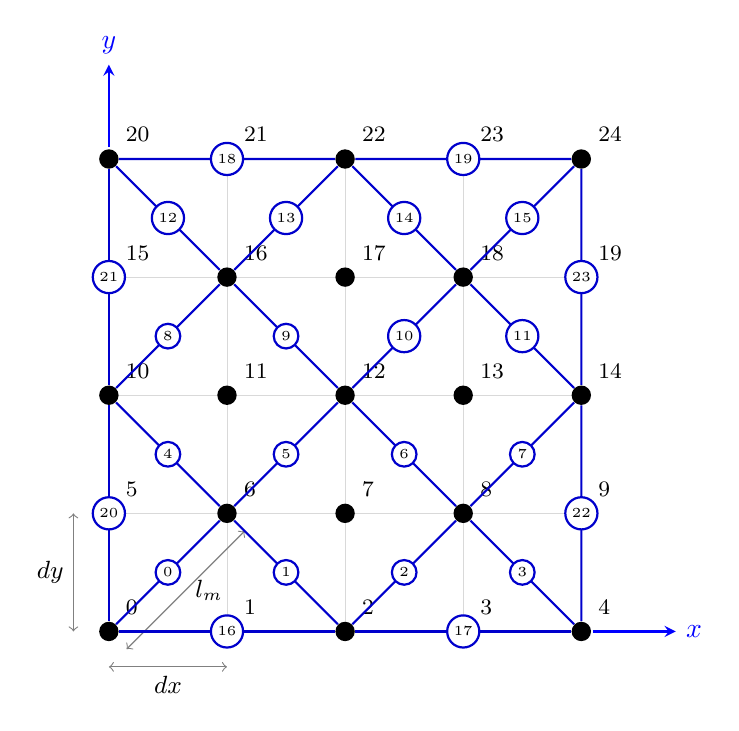
\begin{tikzpicture}[
    scale=1.5, 
    punto/.style={circle, fill=black, inner sep=0pt, minimum size=7pt}, 
    fune/.style={draw=blue!80!black, thick, shorten >=0pt, shorten <=0pt}, 
    asse/.style={->, >=stealth, blue, thick},
    el/.style={circle, draw=blue!80!black, fill=white, font=\tiny, inner sep=1.5pt},
    every label/.style={font=\footnotesize, text=black} 
]

    % 1. Assi cartesiani
    \draw[asse] (4.1,0) -- (4.8,0) node[right] {$x$};
    \draw[asse] (0,4.1) -- (0, 4.8) node[above] {$y$};
    
    % Griglia di sfondo fissa (passo 0.5)
    \draw[gray!30, very thin, step=1] (0,0) grid (4,4);
    
    % Quote passi dx, dy (valgono 1.0 geometrico per n=4, m=4)
    \draw[<->, gray] (0,-0.3) -- (1,-0.3) node[midway, below, black] {\small $dx$};
    \draw[<->, gray] (-0.3,0) -- (-0.3,1) node[midway, left, black] {\small $dy$};
    % Quota della maglia diagonale lm
    \draw[<->, gray] (0.15,-0.15) -- (1.15,0.85) node[midway, right, black] {\small $l_m$};

    % 2. Generazione dei 25 Nodi (Matrice 5x5, da 0 a 24, nx = 5)
    % y = 0
    \node[punto, label={45:0}]  (N0)  at (0,0) {};
    \node[punto, label={45:1}]  (N1)  at (1,0) {};
    \node[punto, label={45:2}]  (N2)  at (2,0) {};
    \node[punto, label={45:3}]  (N3)  at (3,0) {};
    \node[punto, label={45:4}]  (N4)  at (4,0) {};
    % y = 1
    \node[punto, label={45:5}]  (N5)  at (0,1) {};
    \node[punto, label={45:6}]  (N6)  at (1,1) {};
    \node[punto, label={45:7}]  (N7)  at (2,1) {};
    \node[punto, label={45:8}]  (N8)  at (3,1) {};
    \node[punto, label={45:9}]  (N9)  at (4,1) {};
    % y = 2
    \node[punto, label={45:10}] (N10) at (0,2) {};
    \node[punto, label={45:11}] (N11) at (1,2) {};
    \node[punto, label={45:12}] (N12) at (2,2) {};
    \node[punto, label={45:13}] (N13) at (3,2) {};
    \node[punto, label={45:14}] (N14) at (4,2) {};
    % y = 3
    \node[punto, label={45:15}] (N15) at (0,3) {};
    \node[punto, label={45:16}] (N16) at (1,3) {};
    \node[punto, label={45:17}] (N17) at (2,3) {};
    \node[punto, label={45:18}] (N18) at (3,3) {};
    \node[punto, label={45:19}] (N19) at (4,3) {};
    % y = 4
    \node[punto, label={45:20}] (N20) at (0,4) {};
    \node[punto, label={45:21}] (N21) at (1,4) {};
    \node[punto, label={45:22}] (N22) at (2,4) {};
    \node[punto, label={45:23}] (N23) at (3,4) {};
    \node[punto, label={45:24}] (N24) at (4,4) {};

    % 3. ELEMENTI INTERNI (16 Diagonali alternate dall'output per n=4, m=4)
    % j = 0
    \draw[fune] (N0)  -- (N6)  node[midway, el] {0};   % (0+0)%2 == 0 -> SW-NE
    \draw[fune] (N2)   -- (N6)  node[midway, el] {1};   % (1+0)%2 != 0 -> SE-NW
    \draw[fune] (N2)  -- (N8)  node[midway, el] {2};   % (2+0)%2 == 0 -> SW-NE
    \draw[fune] (N4)   -- (N8)  node[midway, el] {3};   % (3+0)%2 != 0 -> SE-NW
    
    % j = 1
    \draw[fune] (N10) -- (N6)  node[midway, el] {4};   % (0+1)%2 != 0 -> SE-NW
    \draw[fune] (N6)  -- (N12) node[midway, el] {5};   % (1+1)%2 == 0 -> SW-NE
    \draw[fune] (N12) -- (N8)  node[midway, el] {6};   % (2+1)%2 != 0 -> SE-NW
    \draw[fune] (N8)  -- (N14) node[midway, el] {7};   % (3+1)%2 == 0 -> SW-NE
    
    % j = 2
    \draw[fune] (N10) -- (N16) node[midway, el] {8};   % (0+2)%2 == 0 -> SW-NE
    \draw[fune] (N12) -- (N16) node[midway, el] {9};   % (1+2)%2 != 0 -> SE-NW
    \draw[fune] (N12) -- (N18) node[midway, el] {10};  % (2+2)%2 == 0 -> SW-NE
    \draw[fune] (N14) -- (N18) node[midway, el] {11};  % (3+2)%2 != 0 -> SE-NW
    
    % j = 3
    \draw[fune] (N20) -- (N16) node[midway, el] {12};  % (0+3)%2 != 0 -> SE-NW
    \draw[fune] (N16) -- (N22) node[midway, el] {13};  % (1+3)%2 == 0 -> SW-NE
    \draw[fune] (N22) -- (N18) node[midway, el] {14};  % (2+3)%2 != 0 -> SE-NW
    \draw[fune] (N18) -- (N24) node[midway, el] {15};  % (3+3)%2 == 0 -> SW-NE

    % 4. ELEMENTI DI BORDO (8 Elementi perimetrali a passo 2)
    % Bordo x in basso
    \draw[fune] (N0)  -- (N2)  node[midway, el] {16};
    \draw[fune] (N2)  -- (N4)  node[midway, el] {17};
    
    % Bordo x in alto
    \draw[fune] (N20) -- (N22) node[midway, el] {18};
    \draw[fune] (N22) -- (N24) node[midway, el] {19};
    
    % Bordo sinistro y
    \draw[fune] (N0)  -- (N10) node[midway, el] {20};
    \draw[fune] (N10) -- (N20) node[midway, el] {21};
    
    % Bordo destro y
    \draw[fune] (N4)  -- (N14) node[midway, el] {22};
    \draw[fune] (N14) -- (N24) node[midway, el] {23};

\end{tikzpicture}